\documentclass[11pt,fleqn]{mythesis}

\usepackage{amsmath}
\usepackage{amsthm}
\usepackage{array}
\usepackage{graphicx}
\usepackage{natbib}
\usepackage{relsize}
\usepackage{caption}
\usepackage{subcaption}  % \begin{subfigure}...\end{subfigure} within figure
\usepackage{multirow}
\usepackage{tabularx}
\usepackage[plainpages=false,pdfborder={0 0 0}]{hyperref}
\usepackage{algorithm}   % \begin{algorithm}...\end{algorithm}

\renewcommand{\listalgorithmname}
{\protect\centering\protect\Large LISTE DES ALGORITHMES}

\usepackage[utf8]{inputenc}
\usepackage[francais]{babel}
\selectlanguage{francais}

%\widowpenalty=10000
%\clubpenalty=10000

\newtheorem{theorem}{\textsc{Theorem}}[chapter]
\newtheorem{definition}{\textsc{Definition}}[chapter]
\newtheorem{example}{\textsc{Example}}[chapter]

\thesistitle{
    Élaboration d'un système de gestion de configuration sensible au contexte
    pour un réseau d'applications.
    %Modèle distribué d’abstraction des informations de contexte, données de
    %configuration et politiques d’administration d’un système de gestion de
    %configuration sensible au contexte dans un reseau d’applications
}

\degreename{Master Recherche Image Informatique et Ingénierie}
\degreefield{Informatique}

\authorname{Ghislain Loaec}
\committeechair{Nader Mbarek}
\othercommitteemembers{Emmanuel Garette}

\degreeyear{2014}
\copyrightdeclaration {
    {\copyright} {\Degreeyear} \Authorname
}

\acknowledgments {
  Je tiens tout d'abord à remercier mon tuteur M. Nader Mbarek pour m'avoir fait
  confiance, puis pour m'avoir guidé, encouragé et conseillé tout en me laissant
  une grande liberté dans la définition et les évolutions du sujet choisi.  Mes
  remerciements vont également à M. Albert Dipanda sans qui ce stage n'aurait
  jamais été possible. Et encore merci à ces messieurs, qui ont accepté d'être
  les rapporteurs de ce mémoire et je les en remercie, de même que pour leur
  participation au Jury.

  Je ne sais comment exprimer ma gratitude à tous les salariés de la société
  Cadoles pour m'avoir permit de menerà bien ce stage dans les meilleurs
  conditions. Je remercie tout particulièrement M. Emmanuel Garette, gérant de
  la société, pour m'avoir suivi tout au long de ce stage et pour la gentillesse
  et la patience qu'il a manifestées à mon égard, ainsi que pour la pertinence
  de ses suggestions.

  Je remercie tous ceux sans qui ce mémoire ne serait pas ce qu'il est :
  aussi bien par les discussions que j'ai eu la chance d'avoir avec eux, leurs
  suggestions ou contributions. Je pense ici en particulier à Daniel Dehennin
  pour les conseils stimulants que j'ai eu le plaisir de recevoir et les
  orientations qu'il a donné à mes lectures.

  Pour leurs encouragements et leur assistance morale, je remercie chaudemment
  ma famille et mes amis. Merci à Mlle. Camille Sintive pour avoir accepté
  d'effectuer un travail de relecture et qui par ses nombreuses remarques et
  suggestions a permis d'améliorer la qualité de ce mémoire, je lui en suis très
  reconnaissant.

  Je remercie de plus tous les auteurs des programmes du domaine public que j'ai
  intensément utilisés durant ce stage, à savoir tous les contributeurs à \TeX,
  \LaTeX, linux, xfig, Zotero et netlib. Sans eux, mes conditions de travail
  auraient sans doute été très différentes et beaucoup moins agréables. Bien que
  je ne les aie jamais rencontrés je remercie aussi E.Summers, D.Kresh et
  G.Higgins, et d'autres dont je ne connais pas le nom, car j'ai profité de leur
  librairie RDFlib qui m'a beaucoup facilité l'approche des ontologies en
  langage Python. Je remercie également M. Lars Otten dont j'ai pillé
  allègrement les formats \LaTeX.

  Enfin, ces remerciements ne seraient pas complets sans mentionner M. Mark
  Burgess, à qui la majorité du travail sur la configuration autonome est due
  qui m'a largement rendu grâce à sa profonde érudition sur le sujet.
}

\newcommand{\mypubentry}[3]{
  \begin{tabular*}{1\textwidth}{@{\extracolsep{\fill}}p{4.5in}r}
    \textbf{#1} & \textbf{#2} \\ 
    \multicolumn{2}{@{\extracolsep{\fill}}p{.95\textwidth}}{#3}\vspace{6pt} \\
  \end{tabular*}
}

\newcommand{\mysoftentry}[3]{
  \begin{tabular*}{1\textwidth}{@{\extracolsep{\fill}}lr}
    \textbf{#1} & \url{#2} \\
    \multicolumn{2}{@{\extracolsep{\fill}}p{.95\textwidth}}
    {\emph{#3}}\vspace{-6pt} \\
  \end{tabular*}
}

\thesisabstract {
  L'objectif fondamental de l'informatique ubiquitaire est de faciliter
  l'utilisation de l'ordinateur. Cela passe par extraire le maximum de bénéfices
  de l'environement numérique. Les défaillances logicielles deviennent monnaie
  courante à mesure que les systèmes informatiques et leur complexité continuent
  de croître. Le problème réside principalement dans l'absence de standards ou
  de modèles réutilisables pour la gestion des informations de contexte. Ce
  mémoire a pour objectif d'apporter un approche simplifiée de la gestion de la
  configuration dans une infrastructure orientée sur les services. Cette
  approche conjugue des concepts tels que les ontologies, la théorie de la
  promesse et le consensus de Raft pour aboutir à un système multi-agents
  tolérant à l'échec.  Les ontologies possèdent un haut degré de formalisme et
  serviront à modéliser les informations de contexte et les politiques de
  comportement. La théorie de la promesse ouvre de nouvelles perspectives sur la
  façon de gérer la configuration, notamment par l'introduction d'une dimension
  sémantique dans la définition de règles de gestion. Enfin l'algorithme de
  consensus de Raft permettra d'abstraire complètement les aspects de
  synchronistation entre les agent, de réplication de l'information et garantit
  une information toujours consistante.
}

% ex: set spelllang=fr spell: %
%%% Local Variables: ***
%%% mode: latex ***
%%% TeX-master: "thesis.tex" ***
%%% End: ***


\hypersetup {
	pdftitle={\Thesistitle},
	pdfauthor={\Authorname},
	pdfsubject={\Degreefield},
}

\setcounter{secnumdepth}{4}

\begin{document}

\preliminarypages

\chapter{État de l'art}

\section{Introduction}

La configuration des composantes logicielles impose un coût majeur dans
l'administration d'un système. Des erreurs de configuration peuvent se traduire
par des vulnérabilités en termes de sécurité, de sévères pertubations dans le
fonctionnement de la brique logicielle, ou purement et simplement provoquer un
déni de service. La prise en considération du contexte pourrait permettre une
abstraction partielle ou complète de cette couche très technique et extrêmement
pénible à configurer.

Un système sensible au contexte doit être capable de mimer la capacité humaine à
reconaître et exploiter l'information implicitement présente dans
l'environement. Cela implique une configuration dynamique de chacune des
composantes de l'architecture, de manière à pouvoir ajuster leur comportement
respectif en fonction de la situation. Identifier l'activité humaine est un
défi, il est essentiel que les applications opèrent en transmettant
l'information appropriée au bon endroit et au bon moment par inférence de
l'intention des utilisateurs. L'infomatique sensible au contexte est un
paradigme dans lequel les application peuvent découvrir et tirer profit d'
informations de circonstance telles que la position actuelle, l'heure de la
journée, les personnes et périphériques dans l'environement et leurs activités.

Dans ce mémoire, nous aborderons les principes communs à chacunes des
architectures existantes, desquels nous detaillerons le framework conceptuel
dérivé (!) par couches. Nous présenterons un certaine variété d'intergiciels et
d'infrastructures reconnus pour faciliter la configuration d'applications et de
services basés sur le contexte.

\section{Background}

De nombreux débats ont eu lieu sur .. Alors que la plupart des gens comprènent
de manière tacite ce qu'est le contexte, ils le trouve par ailleurs
particulièrement difficile à élucider.

... toute information pouvant être utilisée pour caractériser la situation d'une
entité. Une entité peut être une personne, un lieu ou un objet considéré
pertinent dans l'interaction entre un utilisateur et une application, notamment
l'utilisateur et l'application eux même.

Cette définition rend la tâche plus facile à un développeur d'application pour
énumérer le contexte pour un scénario d'application donné. Si un fragment
d'information peut être utilisé pour caractériser la situation d'un participant
dans une quelquonque interaction, alors cette information appartient au
contexte.

\section{Vue d'ensemble sur le contexte}

Le contexte est efficace, seulement lorsqu'il est partagé.

Pour s'assurer que le contexte soit partagé, il doit d'abord être receilli et
rigoureusement traité. Cela implique qu'un système sensible au contexte doit
être en mesure de comprendre ce qu'est le contexte avant d'aller à la recherche
de ces informations et de pouvoir les catégoriser.

\subsection{Classes de contexte}

Schilit et. al. proposent la classification suivante des informations de
contexte:

\begin{itemize}
  \item \textbf{Contexte Informatique} - Connectivité réseau, bande passante,
	  and ressources à proximité telles que des imprimantes, des
	  affichages ou des postes de travail.
  \item \textbf{Contexte Utilistateur} - Le profil utilisateur, sa situation
	  géographique, sa situation sociale actuelle et les individus qui
	  l'entourent.
  \item \textbf{Contexte Physique} - L'éclairage, le niveau de bruit, les
	  condition de circulation ou la température.
\end{itemize}

Chacune de ces catégories contiennent une richesse d'informations pertinantes
pour le système sensible au contexte. Elle ne peuvent cependant pas être
traitées de manière isolée pour pouvoir en extraire le meilleur. L'intention du
système sensible au contexte est de rassembler et de fusionner ces informations
pour aboutir à une vue d'ensemble de la situation. Une fois le contexte mis en
tampon ou en base, le système doit alors filtrer les informations pertinantes
pour l'utilisateur, dans le moment présent.

Les informations de contexte peuvent alternativement être subdivisées en 2
catégories bien distinctes: contexte virtuel ou physique.

\subsubsection{Contexte virtuel}

Le contexte virtuel inclut la version du système d'exploitation, les
possibilités d'interface, la technologie en charge de l'accomplissement des
communications, les emails envoyés et reçus, et les documents édités.

\subsubsection{Contexte physique}

Les contexte physique d'un autre coté peut être la présence d'une autre entité,
qu'elle soit utilisateur ou périphérique, la proximité d'un imprimante en
particulier, une indication que l'utilisateur est debout, en train de marcher ou
assis ou les conditions météorologiques actuelles. En d'autres termes, le
contexte physique peut être défini comme toute donnée aquierable par le biais
d'une sonde.

\subsubsection{Contexte historique}

Les contextes mémorisés au cours d'un certain laps de temps. Cette information
est considérée très utile, mais n'est que très rarement utilisée, sauf pour les
applications mobiles. Le système doit être en mesure d'estimer les informations
valant la peine d'être conservées. Cette évaluation est excessivement coûteuse
et nécéssite donc des algorithmes très performants.

\subsection{Les caractéristiques des informations de contexte}

\subsection{Système sensible au contexte}

\subsection{Recceuillir l'information}

\subsection{Récupérer l'information}

\subsubsection{Capteur en accès direct}

\subsubsection{Infrastructure intergicielle}

\subsubsection{Serveur de contexte}

\subsection{Les achritectures de gestion de contexte}

\subsubsection{Critères d'arbitrages}

\subsection{Représentation du contexte}

\subsection{Interprétation du contexte}

\subsection{Framework conceptuel en couches}

\subsection{Sécurité et confidentialité}

\section{Systèmes et frameworks existants}

\subsection{Technologies de détection}

\subsection{Représentations du contexte}

\subsection{Découverte des ressouces}

\subsection{Gestion du contexte historique}

\subsection{Sécurité et confidentialité}

\subsection{Conclusion}

% This is an example using the \LaTeX{} template for UCI theses and
% dissertation documents \cite{uci-thesis-latex}. Figure
% \ref{fig:sourcecode} is just for illustration purposes, as is Table
% \ref{tab:coordinates}.
% 
% \begin{figure}
% \begin{verbatim}
% #include <iostream>
% int main(int argc, char** argv) {
%   std::cout << "Hello World." << std::endl;
%   return 0;
% }
% \end{verbatim}
%   \caption{Example source code.}
%   \label{fig:sourcecode}
% \end{figure}

\section{Background}

% Lorem ipsum dolor sit amet, consectetur adipisicing elit, sed do
% eiusmod tempor incididunt ut labore et dolore magna aliqua. Ut enim ad
% minim veniam, quis nostrud exercitation ullamco laboris nisi ut
% aliquip ex ea commodo consequat. Duis aute irure dolor in
% reprehenderit in voluptate velit esse cillum dolore eu fugiat nulla
% pariatur. Excepteur sint occaecat cupidatat non proident, sunt in
% culpa qui officia deserunt mollit anim id est laborum.
% 
% \begin{table}
%   \centering
%   \begin{tabular}{|rr|r|}
%     \hline
%     $x$ & $y$ & $z$ \\
%     \hline
%     14 & 12 & -2 \\
%     0 & 33 & -25 \\
%     -3 & 11 & 22 \\
%     4 & 4 & 6 \\
%     \hline
%   \end{tabular}
%   \caption{Example coordinates.}
%   \label{tab:coordinates}
% \end{table}
% 
% Lorem ipsum dolor sit amet, consectetur adipisicing elit, sed do
% eiusmod tempor incididunt ut labore et dolore magna aliqua. Ut enim ad
% minim veniam, quis nostrud exercitation ullamco laboris nisi ut
% aliquip ex ea commodo consequat. Duis aute irure dolor in
% reprehenderit in voluptate velit esse cillum dolore eu fugiat nulla
% pariatur. Excepteur sint occaecat cupidatat non proident, sunt in
% culpa qui officia deserunt mollit anim id est laborum.


%%% Local Variables: ***
%%% mode: latex ***
%%% TeX-master: "thesis.tex" ***
%%% End: ***

\chapter{Problématiques émergentes \newline et orientations de recherche}

Dans ce mémoire, nous avons décrit diverses modèles et principes de conception
d'un système sensible au contexte et présenté une multitude d'intergiciels et
d'approches distribuées pour simplifier la configuration d'applications
sensibles au contexte. De cet état de l'art se dégagent plusieurs problématiques
dans le développement d'un système de configuration basé sur le contexte
auxquelles nous tenterons d'apporter une solution.

\section{Intergiciel et détails d'implémentation}

Le besoin d'un nouvel intergiciel se fait ressentir du coté de l'implémentation.
Les technologies intergicielles actuelles ne sont pas adaptées pour le prise en
considération des restrictions imposées pas la mobilité et les systèmes
environnementaux intelligents : connexions volatiles, traitements et restrictions
mémoire sur les périphériques mobiles, canaux de communication étroits, écrans
réduits, mécanismes d'entrées restreintes, et la liste continue. Il existe
néanmoins une gamme d'implémentations de systèmes sensible au contexte dans la
littérature avec quelques prototypes fonctionnels :

\begin{itemize}
    \item \textbf{Hydrogen} \cite{hofer_context-awareness_2003}: 
        une architecture en trois couches.
    \item \textbf{Gaia} \cite{chetan_mobile_2005}: 
        une autre infrastructure intergicielle, étends les caractéristiques
        génériques des systèmes d'exploitation pour y incorporer la
        sensibilité au contexte.
    \item \textbf{CybreMinder} \cite{abowd_context-aware_2002}: 
        un système sensible au contexte permettant de générer des messages
        de rappel.
    \item \textbf{Context Toolkit} \cite{dey_conceptual_2001}: 
	    une architecture basée sur les widgets.
\end{itemize}

\section{Représentation des informations de contexte}

L'une des principales innovations à apporter dans les infrastructures
d'applications sensibles au contexte réside dans l'introduction d'une interface
présentant un niveau d'abstraction élevé. Cela permettrait de représenter la
connectivité des composants applicatifs avec les politiques de haut niveau qui
la régissent.Cette couche doit rester simple d'utilisation pour les
développeurs d'applications, et le modèle améliorer simultanément
l'automatisation et la sécurité.

\subsection{Ontologie de contexte}

La représentation des informations de contexte est grande préoccupation. Nous
avons présenté dans ce mémoire une approche basée sur les ontologie très
générique. Elle est basée sur quatre concepts fondamentaux : utilisateur,
environnement, plateforme et ressources. Actuellement, les ontologies sont
surtout utilisées pour permettre la communication entre les différents
périphériques dans le même réseau. Comme proposé par le ContextUML
\cite{sheng_contextuml:_2005}, le Langage de Modélisation Unifié (UML) peut
également être utilisé pour modéliser le contexte. Ces modèles pourraient être
utilisés pour séparer la définition et l'information liée au contexte de
l'implémentation spécifique. Il existe d'autres caractéristiques qui font que
l'information de contexte est difficile à modéliser : comme abordé précédemment,
il est parfois nécessaire de différencier une information statique d'une
information dynamique.

\subsubsection{Ontologie de services}

\begin{itemize}
  \item ServiceProfile (partie ''Quoi'')
  \item ServiceModel (partie ''Comment abstrait'')
  \item ServiceGrounding (partie ''Comment concret'')
\end{itemize}

Tout comme pour la standardisation de la gestion intelligente de la
configuration, la classe ServiceModel est très importante. Les services sont
modélisés comme des processus et la classe Process est utilisée pour indiquer
les opérations à des niveaux granularité différents. La classe Process comprend
principalement deux types de processus : atomiques et composites. Puisque
l'information de gestion de configuration est définie comme un ontologie OWL,
l'information peut être utilisée comme les paramètres des opérations de gestion
de la configuration, qui sont définis sous la forme de processus composites.
Chaque service de gestion de configuration correspond à un processus composite,
lui-même composé de plusieurs processus atomiques. Quand le gestionnaire invoque
un service de gestion de configuration prédéfini en OWL-S, le service sera alors
exécuté pour le dispositif réseau en place.

\section{Règles sémantiques et politiques de comportement}

Un autre domaine de recherche concernerait l'utilisation de règles pour exprimer
les comportements souhaités en termes d'éléments de haut niveau. Des langages
de définition de règles sont utilisés dans certains cas pour obtenir la
sensibilité au contexte. CRIME \cite{murphy_coordination_2007} par exemple, est
une implémentation prototypique du modèle Fact Space, qui est un langage de
coordination fournissant aux applications une vue de leur environnement. Les
règles CRIME décrivent le comportement des applications conformément à
l'information de contexte. CRIME traite également les déconnexions en invalidant
les faits et conclusions qui sont tirés des périphériques qui ne sont plus
disponibles dans l'environnement.

\subsection{Gestion basée sur des politiques (Policy-Based)}

La politique est identifiée comme une spécification de la configuration moyenne
du système sur des périodes persistantes. Un aspect important de cette
définition est qu'elle permet une certaine tolérance à l'erreur, nécessitée par
les évènements aléatoires se produisant susceptibles de corrompre la politique
en place dans la boucle de gestion du système. Il existe un élément probabiliste
ou stochastique pour le comportement du système et, par conséquent, la politique
ne peut être qu'une propriété moyenne en général.

\subsection{Théorie de la promesse}

Le modèle permettant la définition des politiques d'administration serait un
modèle orienté sur les ontologies et basé sur la théorie de la promesse.
Celle-ci s'appuie sur un contrôle évolutif des objets intelligents,
contrairement aux modèles impératifs plus traditionnels pensés comme des
systèmes de gestion descendants. Dans ces derniers, le gestionnaire central
doit être informé des commandes de configuration des objets sous-jacents et de
l'état actuel de ces objets.

Au sein du contexte, le modèle fournit une série d'objets qui définissent
l'application. Les objets englobent les terminaux, les groupes de terminaux et
les politiques qui définissent leurs relations.

L'infrastructure conçoit un modèle d'objet pour le déploiement d'applications,
ces dernières constituant le point central. Historiquement, les applications
étaient limitées par les capacités du réseau et par des configurations visant à
prévenir leur utilisation abusive. Des concepts tels que l'adressage, le VLAN et
la sécurité sont depuis toujours intrinsèquement liés, ce qui limite
l'évolutivité et la mobilité des applications. Alors que les applications sont
redessinées pour la mobilité et l'évolutivité web, cette approche traditionnelle
empêche leur déploiement rapide et homogène.

\noindent\rule{8cm}{0.4pt}

La théorie de la promesse est une théorie nouvelle sur ce qu'il peut arriver
dans un réseau de composants entièrement autonomes.

Plutôt que d'adopter la croyance conventionnelle que ''seulement ce qui est
programmé peut arriver'', elle prends le point de vue opposé : ''seulement ce
qui est promis peut être prédit''. Elle aborde donc la gestion du point de vue
de l'incertitude avec réalisme plutôt que celui de la foi en la conformité. Dans
la théorie de la promesse, on suppose un point de vue orienté service des
interactions entre les différents dispositifs informatiques. Chaque nœud propose
de jouer un rôle dans un réseau de collaboration en promettant de restreindre
son comportement de différentes manières. Une utilisation typique de la théorie
de la promesse est d'examiner le comportement en régime permanent d'un certain
nombre d'agents (composants) autonomes. La théorie de la promesse ne détermine
pas nécessairement pleinement le comportement de ses composants, elle représente
seulement les contraintes au sein d'un ensemble de comportements définis. Elle
n'est pas limitée aux promesses linéaires.

La théorie de la promesse adhère à un point de vue orienté service des
politiques des gestion et utilise un langage graphique pour composer et analyser
les propriétés systèmes.

Une caractéristique essentielle des promesses est qu'elles séparent clairement
ce qui contraint et à qui la contrainte s'applique. C'est un autre domaine qui
soulève bien souvent des confusions dans la théorie des politiques. Néanmoins,
le modèle ontologique permet un fois de plus de bien distinguer ces deux
aspects grâce à son haut degré de formalisme.

\subsubsection{Définition de la promesse}

Une promesse est différente d'un engagement : un engagement est le moment où un
agent rompt avec une ligne de conduite pour une autre discontinue avec des vues
sur un objectif, la plupart du temps à travers une action spécifique ou un
investissement sur des résultats futurs. Dans certains cas, l'acte
d'engagement peut résulter en une promesse persistante, mais promettre
n'implique pas une action provoquant un changement discontinu.

\begin{figure}[H]
    \centering
    \begin{tabular}{l}
        ``Une promesse est la spécification d'un état ou comportement \\
        ultérieur d'un agent autonome à un autre. Elle est ainsi, \\
        une unité de politique.`` \cite{burgess_modeling_2006} \\
        \em \footnotesize Mark Burgess, Alva Couch, Modeling Next Generation
        Configuration Management Tools, \\
        \em \footnotesize Pp. 131-147 of the Proceedings of LISA '06,
        Décembre 2006
    \end{tabular}
    \caption{La promesse par Burgess et al. (2006)}
    \label{fig:quote}
\end{figure}

Les promesses sont faites à un agent par un agent et sont modélisées par une
relation unidirectionnelle labellisée par un \emph{corps} de promesse qui
définit la substance de la promesse. Une promesse avec le \emph{corps}
\textbf{+b} est une déclaration pour ''donner'' un comportement d'un agent à un
autre, tandis qu'une promesse avec le \emph{corps} \textbf{-b} est la
spécification de quel comportement sera reçu, accepté ou utilisé d'un agent à
l'autre.

\subsubsection{CfEngine3: une implémentation de référence de la théorie de la
promesse}

CfEngine3 implémente deux approches :

\begin{itemize}
    \item \textbf{Centralisée}: 
        le système va pousser avec force les règles et règlements établis de
        manière centralisée avec ou sans la volonté de l'utilisateur final hôte.
    \item \textbf{Basé sur des politiques} :
        cette approche fonctionne de la même manière que le protocole SNMP
        (Simple Network Management Protocol), à l'exception qu'elle donne une
        autonomie totale aux agent, de manière à ce qu'ils aient plein droit de
        tirer et implémenter un ensemble centralisé de politiques de
        configuration.
\end{itemize}

En théorie, chacun des agents autonomes va faire formuler une promesse sur le
comportement qu'on attend de lui, basé sur un choix qui lui est propre. C'est ce
que rend la théorie de la promesse optimale pour un framework de gestion basé
sur des politiques.

La théorie de la promesse décrit des services régies par des politiques, dans un
framework d'agents complètement autonomes, qui s'aident les uns les autres
seulement par une coopération volontaire. Dans CfEngine3, chaque élément de
configuration va faire une promesse concernant ses caractéristiques propres et
sa relation avec d'autres éléments de configuration.

Nous souhaitons être en mesure de promettre que le système est cohérent, de le
vérifier et d'effectuer des changements seulement si nos promesses ne sont pas
tenues. Cela nécessite, en plus de l'implémentation initiale de ces promesses,
la vérification continue de l'état de chacun des éléments de configuration
vis-à-vis de leur promesses respectives pour assurer un système cohérent et en
conformité avec les politiques en vigueur.

% TODO : expliquer ITIL
%Pour comprendre ITIL (Information Technology Infrastructure Library), il
%faut l'imaginer comme un service fourni par CfEngine.

\subsubsection{Processus de raisonnement lié à la promesse}

Le procédé de raisonnement qui accompagne l'émanation d'un promesse, se divisent
en plusieurs sous-étapes, accrochez-vous:

\begin{itemize}
  \item \textbf{Préparation de la promesse} :
	Processus de raisonnement effectué par A conduisant à la conception, la
	synchronisation et la délivrance de la promesse P par A.
  \item \textbf{Analyse de crédibilité} :
	Processus de raisonnement où les agents C dans le champ d'application de
	la promesse P déterminent la crédibilité qu'ils assignent à A promettant
	P compte tenu des faits connus de A (mais à l'exception des informations
	historiques précises sur le comportement individuel d'un membre de sa
	classe d'agent)
  \item \textbf{Détermination préliminaire de la confiance} :
	Processus de raisonnement effectué par C (C dans le domaine
	d'application de la promesse P) servant à :
  	\begin{enumerate}
	  \item Déterminer la confiance que C accorde à A avant même de
		  connaitre la promesse P (confiance préalable)
	  \item Spécifier quelles sont les attentes générées par la prise en
		  considération de la promesse P.
  	\end{enumerate}
  \item \textbf{Délibération de contre-promesse} :
	Processus de raisonnement effectué par B concernant les contre-promesses
	pouvant potentiellement être émises par B en retour de considération de
	P (B dans le champ d'application de P)
  \item \textbf{Prédiction de l'impact de la promesse} :
	(cela peut être réalisé à condition que B ait émis une ou plusieurs
	contre-promesses plausibles)
  	\begin{enumerate}
	  \item Processus de raisonnement effectué par B (dans le champ
		  d'application de P) et C (n'importe quel agent dans le champ
		  d'application de P) servant à déterminer les (le changement
		  des) attentes que P créé dans B (et que A a l'intention de
		  générer).  
	  \item Processus de raisonnement visant à la modification des ententes
		  (détenues par B ou C) étant donné la changement des attentes
		  de chacun d'entre eux amené par la prise en considération de
		  la promesse P.
  	\end{enumerate}
  \item \textbf{Évaluation de la promesse} :
	Processus de raisonnement effectué par C concernant :
  	\begin{enumerate}
	  \item La façon dont C va évaluer si la promesse de A a été tenue ou
		  non.
      \item L'évaluation de cette dernière au moyen de la méthode la plus
          adéquate
  	\end{enumerate}
  \item \textbf{Surveillance de rétraction de promesse} :
	A peut être amené à un stade ultérieur à émettre une autre promesse Q,
	pour laquelle la tenue n'est pas compatible avec la tenue de P. Dans ce
	cas, Q qualifie un retrait de P. Un agent C applique un processus de
	raisonnement qui surveille et évalue les promesses postérieures émises
	par A pour déterminer si celles-ci seront amenées à rompre la promesse P
	et induire sont retrait.
  \item \textbf{Mise à jour de la confiance} :
	Processus de raisonnement en place pour chacun des agents C dans le champ
	d'application de P visant à mettre à jour la confiance préalablement
	accordée à A, en adéquation avec la résultat de l'évaluation que C fait
	concernant le degré avec lequel la promesse P a été tenue par A.
  \item \textbf{Critère de réputation} :
	Processus de raisonnement effectué par chacun des agents C dans le champ
	d'application de P visant à échanger entre les différent agents les
	effets des mises à jour de confiance. Le flux de réputation permet a un
	agent C n'ayant aucuns aprioris sur un agent A d'acquérir une confiance
	initiale en prenant en considération les preuves recueillies par les
    autres agents (parce que même les agents ont des casiers judiciaires).
\end{itemize}

\subsubsection{$\pi$-calculus}

TODO or NOT TODO, that is the question

\section{Consistance de l'information et tolérance à l'échec}

\subsection{Algorithme de consensus de Raft}

Le consensus est un problème fondamental dans les systèmes distribués tolérants
aux pannes. Un consensus implique de multiples serveurs acceptant des valeurs.
Une fois qu'ils atteignent une décision sur une valeur, cette décision est
définitive. Les algorithmes de consensus typiques sont amenés à faire des
progrès lorsque la majorité de leurs serveurs sont disponibles, par exemple, un
cluster de 5 serveurs peut continuer à fonctionner même si deux serveurs ne sont
plus disponibles. Si plusieurs serveurs échouent, ils cessent de faire des
progrès (mais ils ne retournerons jamais de valeurs erronées).

Raft est un algorithme de consensus qui est conçu pour être facile à comprendre.
Il est équivalent à Paxos dans la tolérance aux pannes et en termes de
performance. La différence est qu'il est décomposé en sous-problèmes
relativement disjoints, et traite de manière rigoureuse toutes les pièces
majeures nécessaires pour obtenir un système cohérent.

\subsubsection{Architecture de machines à états répliquées}

\begin{wrapfigure}{r}{.5\textwidth}
    \centerline{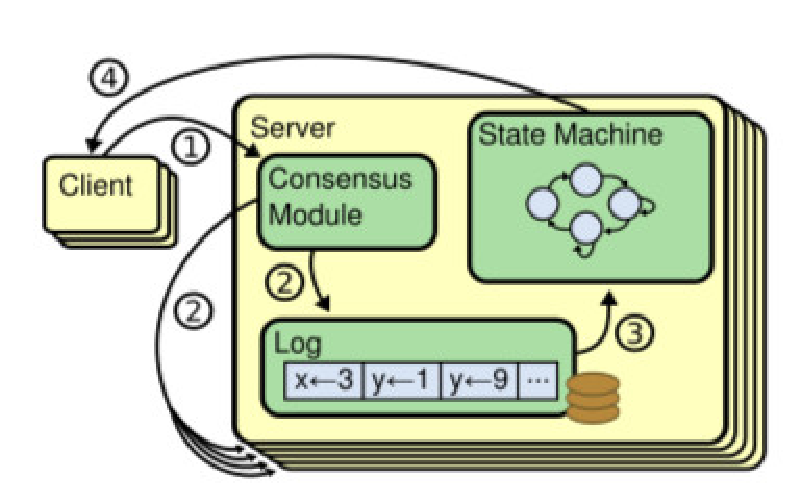
\includegraphics[width=.47\textwidth]{img/replicated_state_machine}}
    \caption{Procédé de réplication des machines à états}
    \label{replicated_state_machine}
\end{wrapfigure}

L'algorithme de consensus gère un registre répliqué contenant les commandes de
la machine à états de chacun des clients dans le réseau. Les machines à états
traitent des séquences identiques de commandes à partir de journaux partagés, de
sorte qu'ils produisent les mêmes résultats.

Les systèmes à grande échelle n'ayant qu'un seul cluster leader utilisent une
machine à état distincte pour gérer les élections et pour stocker les
informations de configuration qui doivent survivre aux crashs du leader
(exemple: Chubby, ZooKeeper).

\begin{verse}
    \underline{
        Garder le registre répliqué consistant est le travail de l'algorithme de
        consensus.
    }
\end{verse}

Les algorithmes de consensus pour les systèmes concrets ont généralement les
caractéristiques suivantes :

\begin{itemize}
    \item Ils assurent la sécurité (ne retournent jamais de résultat erroné)
        sous toutes conditions non byzantines, y compris les retards dans le
        réseau, les pertes de partitions et de paquets, la duplication et
        la réorganisation.
    \item Ils sont entièrement fonctionnels (disponibles) dans la mesure où au
        moins la majorité des serveurs sont opérationnels et peuvent communiquer
        avec les uns les autres et avec les clients. Ainsi, un groupe type de
        cinq serveurs peut tolérer la défaillance de deux ses membres. Les
        serveurs sont supposés tomber en panne en s'arrêtant ; ils pourront plus
        tard retrouver un état stable et rejoindre le cluster.
    \item Il ne dépendent pas de la contrainte temporelle pour assurer la
        cohérence des journaux : des horloges défectueuses et des retards
        abusifs dans la délivrance des messages peuvent causer des problèmes de
        disponibilité. 
    \item Dans le cas le plus courant, une commande peut s'achever aussitôt que
        la majorité de la grappe a répondu à un seul tour d'appels à procédures
        distantes ; une minorité de serveurs lents de doivent pas impacter les
        performances globales du système.
\end{itemize}

\subsubsection{États des serveurs}

Un cluster Raft comprend une multitude des serveurs (cinq est un nombre courant
permettant au système de tolérer deux échecs). À n'importe quel moment donné,
chacun des serveur est dans l'un de ces états :

\begin{wrapfigure}{r}{.5\textwidth}
    \centerline{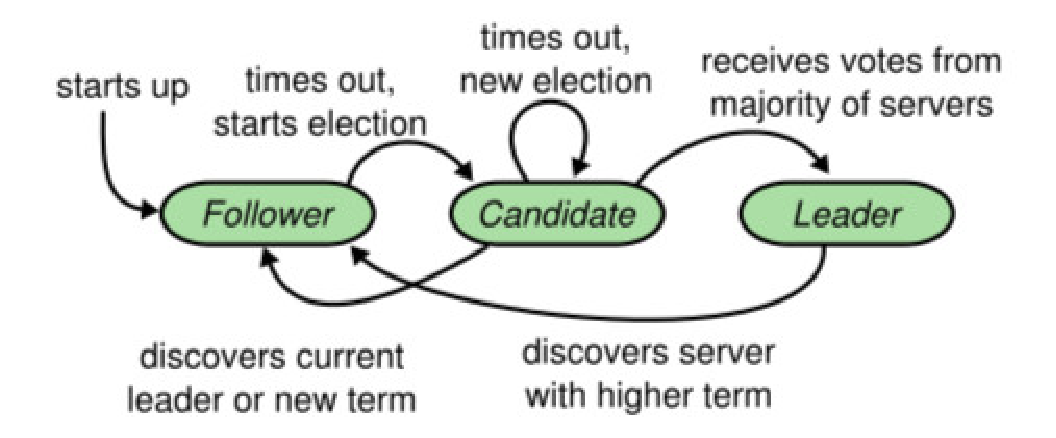
\includegraphics[width=.47\textwidth]{img/raft_server_states}}
    \caption{États et transitions dans un cluster Raft}
    \label{raft_server_states}
\end{wrapfigure}

\begin{itemize}
    \item \textbf{Leader} :
        En cycle normal, il existe un et un seul \emph{leader} et tous les autres
        serveurs sont \emph{followers}. Le \emph{leader} traite les requêtes de
        tous les clients (si un client contact un \emph{follower}, le
        \emph{follower} le redirige vers le \emph{leader}).
    \item \textbf{Follower} :
        Les \emph{followers} sont passifs : ils n'émettent jamais de messages par
        leur propre initiative, ils se contentent simplement de répondre aux
        requêtes émises par le \emph{leader} et les \emph{candidats}.
    \item \textbf{Candidat} :
        Statut intermédiaire utilisé lors de l'élection d'un nouveau
        \emph{leader}. La figure \ref{raft_server_states} montre les différents états
        et transitions possibles dans le consensus de Raft.
\end{itemize}

% ex: set spelllang=fr spell: %
%%% Local Variables: ***
%%% mode: latex ***
%%% TeX-master: "thesis.tex" ***
%%% End: ***

\chapter{Simulation}

\begin{figure}
  \begin{verbatim}
  #include <iostream>
  int main(int argc, char** argv) {
    std::cout << "Hello World." << std::endl;
    return 0;
  }
  \end{verbatim}
  \caption{Example source code.}
  \label{fig:sourcecode}
\end{figure}

\section{Conclusion}

Component technologies will play a fundamental role in the next generation
computer systems as the complexity of software and the diversity and
pervasiveness of computing devices increase. However, component technologies
must offer mechanisms for automatic management of inter-component dependencies
and component-to-resource dependencies. Otherwise, the development of
component- based systems will continue to be difficult and frequently lead to
unreliable and non-robust systems.  

Future ubiquitous computing environments will be composed of thousands of
devices running millions of software components. Current systems rely heavily
on manual configuration but with a system composed of millions of components
this will no longer be possible.  There are only two ways out of this
situation: static configuration or dynamic, automatic configuration

Since future environments tend to be more and more dynamic, automatic
configuration seems to be the only viable solution.


\clearpage
\phantomsection

\bibliographystyle{abbrv}
\bibliography{thesis}

\captionsetup[figure]{list=no}
\captionsetup[table]{list=no}

% The original template (from Trevor) had a custom \appendix command,
% but I found it to break figure/table counters. I'm not sure how
% reliable my fix is, so I ended up reverting back to the standard
% latex version, and renaming the custom command to \myappendix.  You
% can try both and see how things work out:
% 1) Call \appendix once, and then make each appendix a \chapter
% 2) Call \myappendix once, and then make each appendix a \section.

\appendix

\chapter{Ontologie de contexte}
\label{appendix:ontology}

\section{Entités de l'ontologie}

\begin{itemize}
  \item \textbf{Machine} est n'importe quel périphérique en mesure d'accepter et
	  de traiter des informations pour fournir le résultat désiré basé sur
	  un programme ou une séquence d'instructions sur comment les données
	  doivent être traitées.
  \item \textbf{Computers} sont le type principal de machines dans cette étude.
	  C'est pourquoi les deux terminologies sont interchangeables dans
	  diverses sections de ces travaux. Les ordinateurs personnels (PCs),
	  les ordinateurs portables et les serveurs héritent tous de ce type.
  \item \textbf{Operating System} est un programme faisant le pont en les
	  composants logiciels et les composants matériels sous-jacents d'une
	  machine. Le système d'exploitation est une entité comportant plusieurs
	  sous-classes disjointes telles que Windows XP, OS X ou Linux.
  \item \textbf{Packages} sont les programmes applicatifs conçus pour servir un
	  but spécifique comme distribuer un service local, réseau ou web sur
	  une ou plusieurs machines. Le paquet Apache est en bon exemple
	  d'entité conçue pour activer un service web.
  \item \textbf{Service} est une fonctionnalité spécifique d'un système
	  informatique comme un service web ou réseau offert par une machine. Un
	  processus qui est défini dans ce document comme un ensemble ou d'une
	  partie d'un ensemble de mesures permettant la fourniture de services
	  en exécutant des activités réelles en tâche de fond.
  \item \textbf{Command} est un utilitaire pouvant être utilisé par les
	  utilisateurs pour démarrer un processus spécifique, à la condition
	  qu'il n'existe pas de planification pour l'exécution de cette même
	  tâche. Un très bon exemple permettant d'illustrer cette relation
	  entre ces deux entités serait un web service, qui nécessite qu'un
	  processus tel que ''httpd'' soit démarré en arrière plan à l'aide de
	  la commande ''\begin{verbatim}httpd start\end{verbatim}''.
  \item \textbf{Storage} est une partition logique d'un média de stockage
	  physique qui sert principalement d'hôte pour les différents types de
	  fichiers. Un fichier est défini comme une collection d'informations
	  complète comme un programme, un ensemble de données utilisées par un
	  programme ou un document créé par un utilisateur.
  \item \textbf{Interface} est défini comme un périphérique permettant l'accès à
	  un réseau par une machine.
\end{itemize}

\section{Propriétés objets de l'ontologie (Relations)}

\begin{itemize}
  \item \textbf{Caused By} :
          Un type d'association où une entité joue le rôle d'affecter l'autre en
	  changeant son état de l'état X à l'état Y.
  \item \textbf{Configured By} : 
	  Quand une entité X peux apporter les changements nécessaires à
	  l'entité Y pour lui permettre d'accomplir ses objectifs et ses
	  intentions. Le lien entre une machine et un progiciel de gestion de
	  configuration comme CfEngine 3 est un exemple typique de ce type de
	  relations.
  \item \textbf{Edited By} : 
	  Décrit qu'un fichier peut être modifié par un éditeur tel que
	  l'utilisateur du fichier à certaines fins.
  \item \textbf{Managed By} : 
	  Si X est responsable du bon fonctionnement de Y dans l'accomplissement
	  de son objectif, X est dit manager de Y. Le fait qu'une entité hérite
	  de ce rôle implique une supervision constante et des prises de mesures
	  lorsqu'intervient une déviation dans le comportement souhaité.
  \item \textbf{Monitoring By} : 
	  La supervision est principalement la responsabilité de garder un œil
	  sur quelque chose. Si une entité X supervise Y, elle surveille une
	  quelconque altération de comportement pour en informer le ou les
	  managers en charge de cette entité.
  \item \textbf{Component Of} : 
	  La relation entre une entité X, composant d'une entité plus globale Y
      qui joue le rôle d'encapsuleur pour ce composant X.
  \item \textbf{Owned By} : 
	  La propriété est un type de relation pouvant exister entre entité
	  devenue possession et son propriétaire. Le lien entre un fichier et son
	  propriétaire est un exemple de cet type d'association.
  \item \textbf{Promised By} : 
	  La relation en une promesse et l'entité qui la formule. 
  \item \textbf{Required By} : 
	  Si X dépend de Y dans l'accomplissement de ses intentions, la relation
	  entre ces deux entités est de type ''Required By''.
  \item \textbf{Runs On} : 
	  Si l'entité X exerce ses activités ou son exécution sur l'entité Y, la
	  relation est appelé ''Runs On''.
  \item \textbf{Written By} : 
	  La relation entre une écriture X et son auteur Y.
  \item \textbf{Used By} : 
	  Si une entité X fait l'usage d'une entité Y à n'importe quelle moment
	  de son exercice, la relation est de type ''Used By''.
  \item \textbf{Started By} : 
	  Quand une entité X est responsable du démarrage d'une entité Y ou
	  qu'elle commence à se comporter d'un certaine manière, l'association
	  est dite de type ''Started By''.
  \item \textbf{Provided By} : 
	  Quand une entité X a le potentiel et la bonne volonté de fournir
	  quelque chose à une autre entité Y, la relation entre ces deux entités
	  est appelée ''Provided By''.
  \item \textbf{Installed By} : 
	  Une entité X peut mettre en place un programme Y dans une machine de
	  manière à accomplir son but recherché. La relation existante entre X
	  et Y est alors de type ''Installed By''.
  \item \textbf{Contained In} :
	  Si une entité X est contenue dans Y, physiquement ou conceptuellement,
	  la relation est de type ''Contained In''.
\end{itemize}

\section{Propriétés de données de l'ontologie (Attributs)}

\begin{itemize}
  \item \textbf{AllowConnectFrom} : Liste d'adresses IP ou de nom d'hôtes
	  susceptibles d'avoir plus d'une connexion au port d'un serveur.
  \item \textbf{CheckForeign} : Indique s'il est nécessaire de vérifier les
	  autorisations sur le répertoire racine lors de la recherche de la
	  profondeur.
  \item \textbf{CheckRoot} : Liste de nom d'hôtes ou d'adresses IP auxquels
	  accorder un droit de lecture sur le serveur.
  \item \textbf{ForceIpv4} : Indique s'il y a un usage forcé de l'adresse IP
	  pour les connexions.
  \item \textbf{IsMachineVirtualized} : Indique si une machine est virtuelle ou
	  non.
  \item \textbf{PackageFileRepository} : Liste de répertoires locaux à la
	  machine pour la recherche de paquets.
  \item \textbf{TrustKeyFrom} : liste des hôtes pour lesquelles une machine
	  acceptera les clés publiques sur base de la confiance. Définition des
	  types d'occurrences qui sont liés avec le type d'entité stockage sont
	  répertoriés ci-dessous. Un stockage est une partition logique d'un
	  support de stockage physique.
  \item \textbf{FreeSpace} : Pourcentage minimum ou absolu d'espace disque
	  devant être disponible sur le support de stockage avec de lever un
	  avertissement.
  \item \textbf{MountType} : Type de protocole d'un système de fichier distant. 
  \item \textbf{FileSystemFlag} : Liste des options de menu à définir pour les
	  drapeaux de système de fichiers BSD. 
  \item \textbf{Atime} : Plage temporelle d'accès pour les fichiers
	  admissibles.
  \item \textbf{SecureInput} : Indique si les fichiers d'entrée sont accessibles
	  en écriture pour les utilisateurs non-autorisés.
  \item \textbf{MountType} : L'option de menu pour le type de liens à utiliser
	  lors de la copie comme le lien symbolique et le lien physique.
  \item \textbf{AuditingEnabled} : Indique si la fonctionnalité de journal
	  d'audit d'un paquet est activé ou non.
  \item \textbf{LogLevel} : Le niveau de rapport envoyé à syslog.
  \item \textbf{Architecture} : L'architecture relative à la section de paquets
	  comme ''x86-64'' ou ''i386''.
  \item \textbf{BuildsOn} : Liste de groupement de promesses sur lesquelles
	  s'appuie ou dépend une promesse d'une certaine manière (pour la
	  gestion des connaissances)
  \item \textbf{HomeDirectory} : Répertoire contenant les fichiers personnels
	  d'un utilisateur.
  \item \textbf{ShellAccount} : Compte personnel donnant accès à une invite de
	  commande Unix.
  \item \textbf{Module} : Indique s'il faut s'attendre à un protocole de module
	  CfEngine.
\end{itemize}

\chapter{Interface d'administration}
\label{appendix:interface}

\begin{figure}[H]
    \centerline{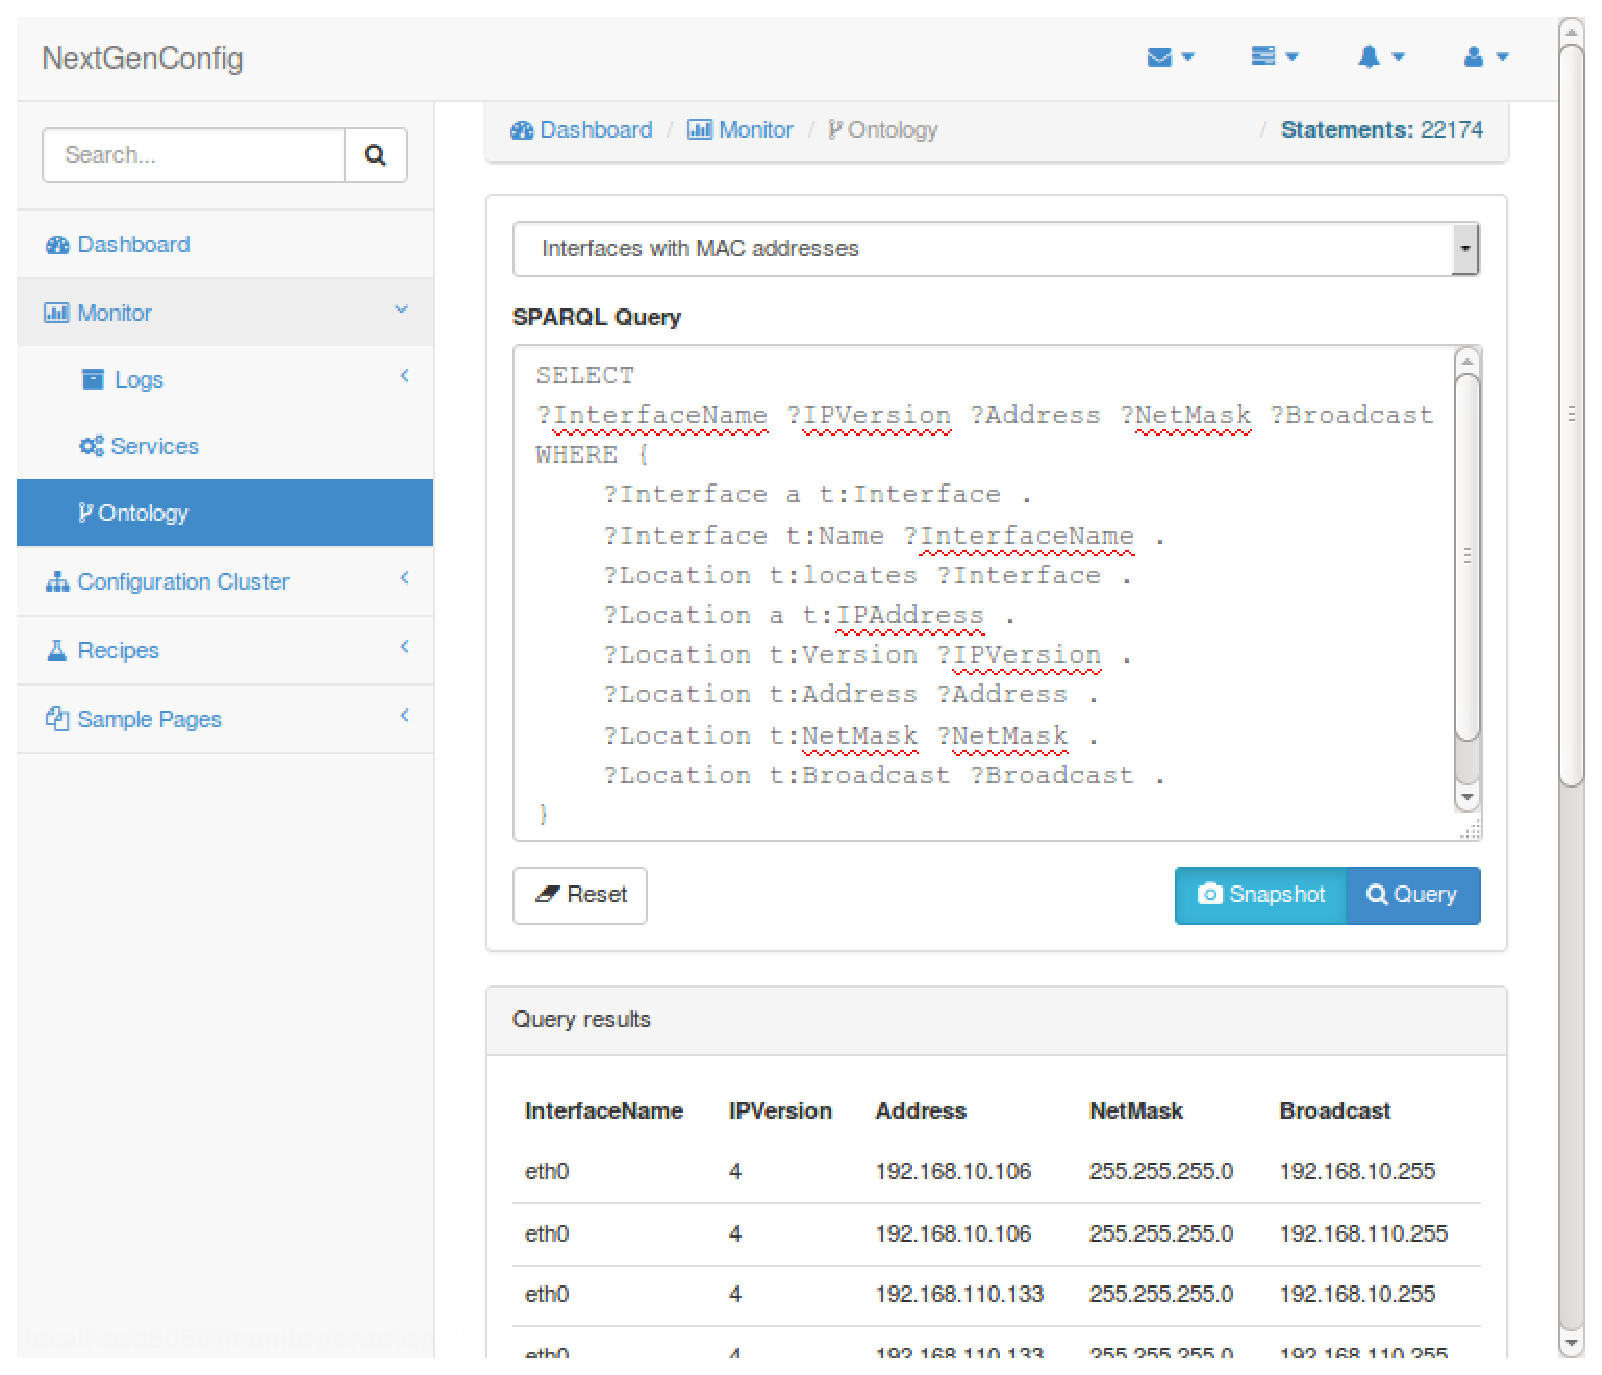
\includegraphics[width=\textwidth]{img/trifle_gui}}
    \caption{Interface d'administration du gestionnaire de configuration}
    \label{fig:trifle_gui}
\end{figure}

% ex: set spelllang=fr spell: %
%%% Local Variables: ***
%%% mode: latex ***
%%% TeX-master: "thesis.tex" ***
%%% End: ***


\end{document}
